\section{Durchführung und Auswertung}
In unserem Versuch vermessen wir nun unsere Germanium-Probe im Temperaturbereich -180 bis 40 $^{\circ}C$ also von $\approx 90$ bis $\approx 315 K$. Mit der Van-der-Pauw-Methode messen wir also die entstehenden Spannungen bei einem Probenstrom von $1mA$ und berechnen daraus die temperaturabhängigen Verläufe von spezifischem Widerstand, Hall-Konstante und Ladungsträgerdichte. Für die Temperaturen verwenden wir die gemessene Temperaturspannung, wobei wir den Mittelwert aus den Spannungen vor und nach der Aufnahme eines Messwerts verwenden. Die genaue Temperatur ergibt sich aus der gemittelten Spannung über einen Fit 5.Grades, welcher zur Veranschaulichung in Abbildung \ref{temp} dargestellt ist.

\begin{figure}[htbp] 
     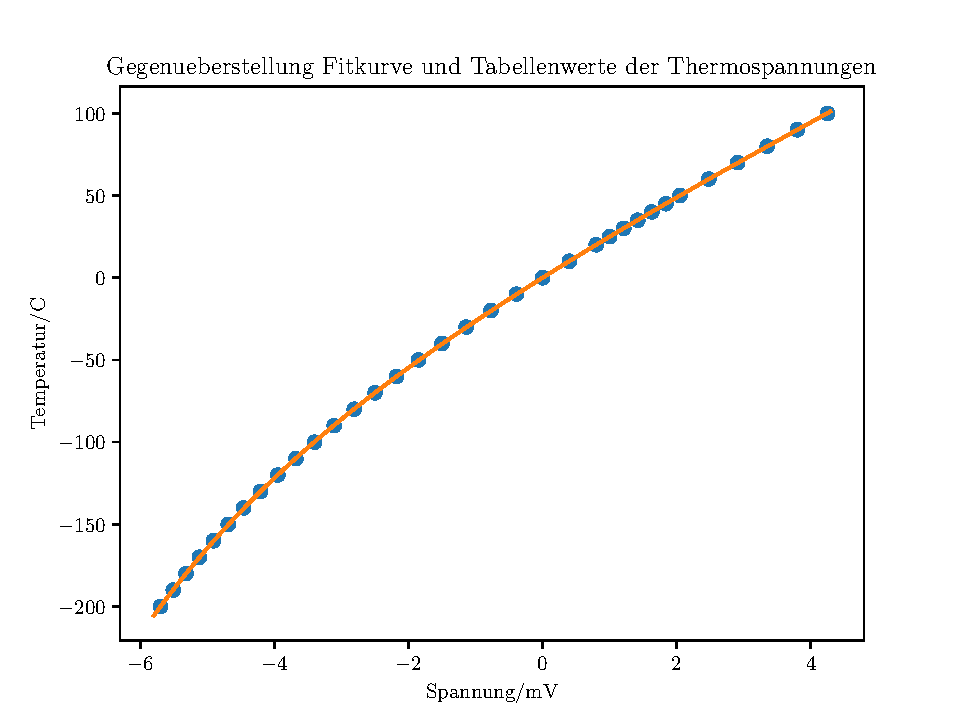
\includegraphics[scale=0.7]{temp_fit.pdf}
  \caption{Temperaturfit der Temperaturspannung}
  \label{temp}
\end{figure}

Aus den Messwerten direkt ersichtlich ist das negative Vorzeichen der Hall-Konstante, woraus die Dotierung als n-Dotierung identifiziert werden kann.

Die Verläufe der Größen $R_H$, $n$ und $\rho$ sind in den Abbildungen \ref{hall} bis \ref{n} logarithmisch gegenüber $\frac{1}{T}$ dargestellt. Für die Berechnung des spezifischen Widerstands wurde dabei ein konstanter Wert von $f=0.97$ für den Korrekturfaktor verwendet. 

\begin{figure}[htbp] 
     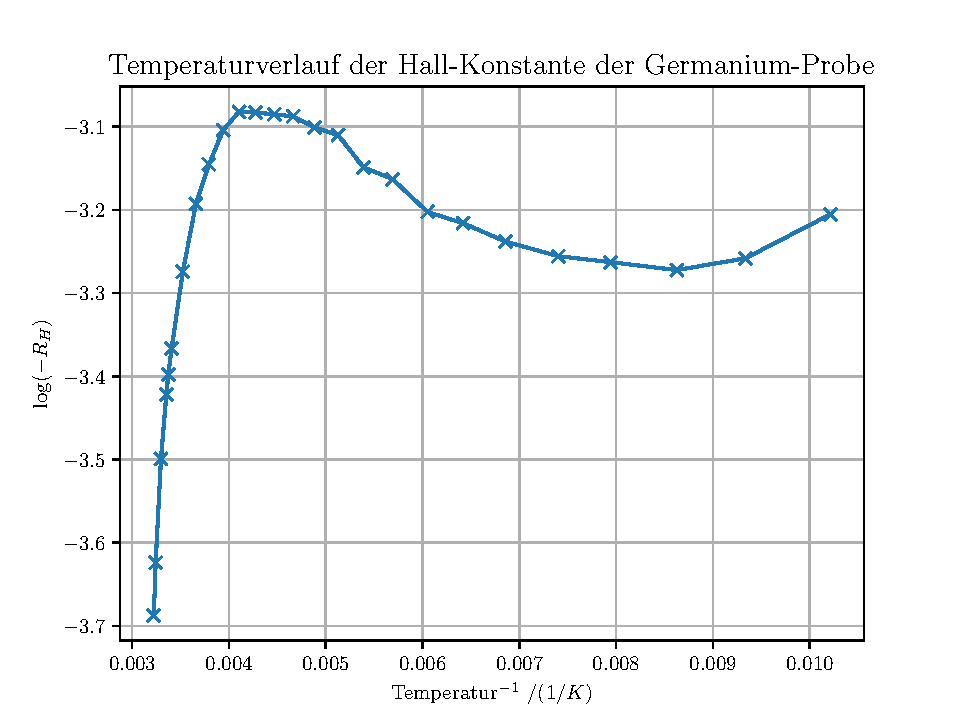
\includegraphics[scale=0.7]{temp_hall.pdf}
  \caption{Temperaturverlauf der Hall-Konstante}
  \label{hall}
\end{figure}

\begin{figure}[htbp] 
     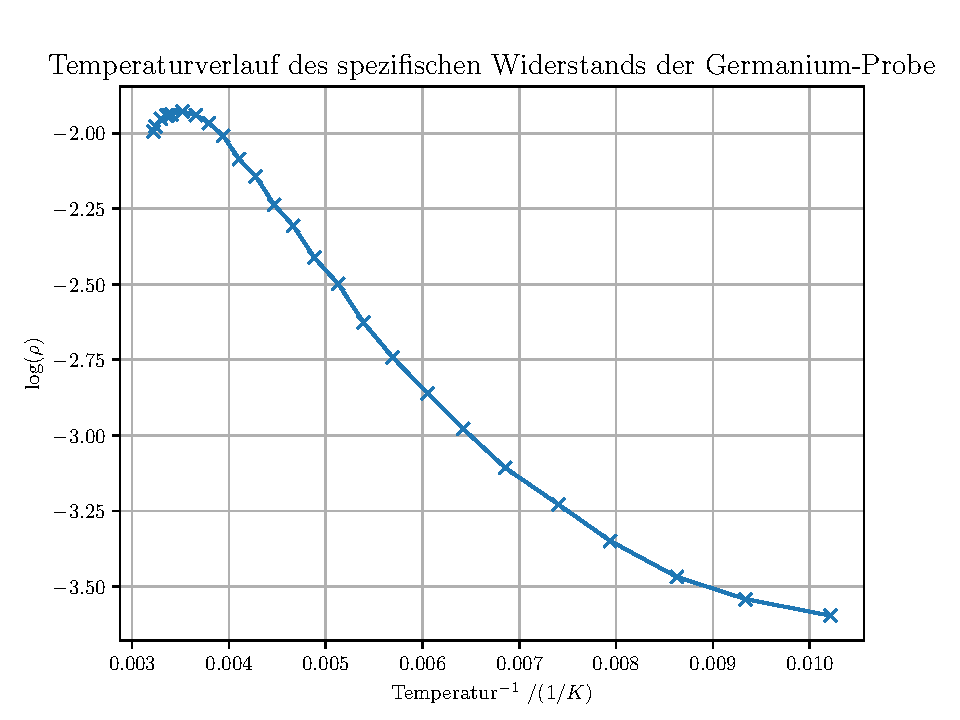
\includegraphics[scale=0.7]{temp_rho.pdf}
  \caption{Temperaturverlauf des spezifischen Widerstands}
  \label{hall}
\end{figure}

\begin{figure}[htbp] 
     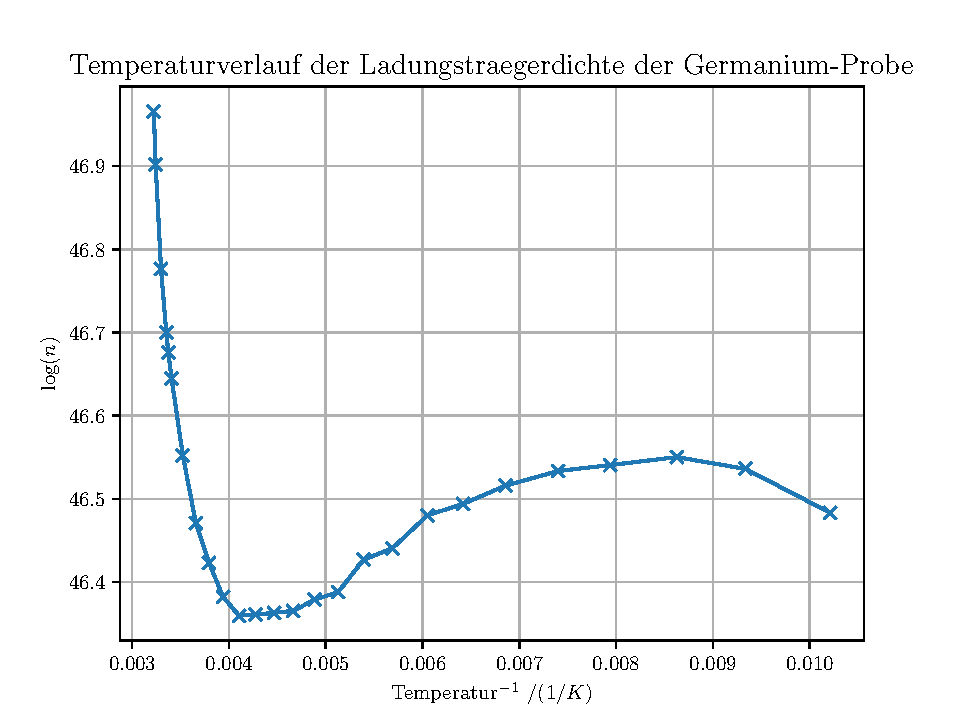
\includegraphics[scale=0.7]{temp_n.pdf}
  \caption{Temperaturverlauf der Ladungsträgerdichte}
  \label{n}
\end{figure}


Unsere Ladungsträgerdichte n weist im hohen Temperaturbereich das charakteristische exponentielle Verhalten auf und steigt rasant an. Im mittleren Temperaturbereich erwarten wir einen konstanten Verlauf der Ladungsträgerdichte, wohingegen wir einen leichten Anstieg messen. Dies ist physikalisch unsinnig, da bei niedrigerer Temperatur natürlich auf keinen Fall mehr Ladungsträger im Leitungsband vorhanden sein sollten, sondern die Ladungsträgerdichte aufgrund der Störstellenerschöpfung konstant sein sollte. Hin zu besonders niedrigen Temperaturen sinkt die gemessene Ladungsträgerdichte wiederum ab, was aufgrund der Anhebung von immer weniger Elektronen ins Leitungsband auch so zu erwarten war. 
Bei Betrachtung unserer Messwerte muss allerdings auch die sehr hoch aufgelöste Skala beachtet werden, sodass unsere Schwankungen im konstant erwarteten Bereich im Vergleich besonders zu den sehr stark steigenden Messwerten im Hochtemperaturbereich nicht sehr stark ins Gewicht fallen. Da weiterhin die Tief- und Mitteltemperaturmessung mit sehr schnell steigenden Temperaturen durchgeführt wurden, sind die Messwerte mit Vorsicht zu genießen und weisen vermutlichen einen hohen Fehler auf.


Aus den Messergebnissen kann man weiterhin noch die Beweglichkeit der Elektronen in Germanium berechnen. Es gilt nämlich für die Leitfähigkeit:

\begin{align}
\sigma=ne\mu
\end{align}

Daraus folgt für die Beweglichkeit:

\begin{align}
\mu=\frac{1}{ne\rho}
\end{align}

Die Beweglichkeit ist ebenfalls temperaturabhängig und in Abbildung t doppelt logarithmisch dargestellt.